\chapter{Theoretical background }\label{sec:theory}

\section{The learning framework}

Statistical learning theory encompasses the mathematical framework used to
study generalization in machine learning
\cite{n.vapnikNatureStatisticalLearning2000}.
In this formalism, the goal
is to learn a target function $f^*: \mathcal{X} \longmapsto \mathcal{Y}$ 
by means of an approximated function $f \in \mathcal{F}$ using a 
finite set of observations. 

\begin{definition}[\emph{Supervised dataset}]\label{def:dataset}
    Let $\mathcal{X}$ and $\mathcal{Y}$ be
    the input and output spaces of the target function $f^*$, respectively. Let $X$ 
    be a random variable associated with a sampling experiment in the input space, thus 
    defining a measure of probability $P_X$ with support $\mathcal{X}$.
    Let $\bm{X} = (X_1, ..., X_N)$ be a (simple)
    random sample of $X$ with size $N$ \cite{casellaStatisticalInference2002}.
    A supervised dataset $D$ is constructed from a realization
    $\bm{x} \sim \bm{X}$ by pairing each observation $x$ with its corresponding
    value $f^*(x)$ under the target function:

    $$
    D = \{(x_n, f^*(x_n))\}_{n \in [N]}.
    $$
    % (\bm{x}, \bm{f^*}(\bm{x})) 

    The class of supervised datasets generated from $\bm{X}$ will be denoted by $\mathcal{D}$.
    % We will use $\mathcal{D}$ to refer to the class of supervised datasets generated from $\bm{X}$.
    % In general, $\mathcal{D}$ will represent the class of supervised datasets generated from $\bm{X}$.
\end{definition}

\begin{definition}[\emph{Empirical risk}]\label{def:erm}
    Let $D$ be a supervised dataset generated from a sample $\bm{x} \sim \bm{X}$. 
    Let $L: \mathcal{Y} \times \mathcal{Y} \longmapsto \mathbb{R}$ be a loss function 
    measuring the discrepancy at observation $x \in \bm{x}$ between the prediction of the model $f(x)$ and 
    its corresponding true value $f^*(x)$. The overall quality of the approximation $f$ can be 
    measured with its expected risk $R(f)$:

    $$
    R(f)=\mathbb{E}_{X} L(f(x),f^\star(x)).
    $$

    We can approximate the expected risk with its empirical (plug-in)
    analogous if $N$ is large enough (see Glivenko-Cantelli 
    theorem \cite{gutIntermediateCourseProbability2009}).
    The empirical risk of $f \in \mathcal{F}$ computed on $D$ is defined as

    $$
    \hat{R}(f)=\frac{1}{N}\sum_{n=1}^{N}L(f(x_{n}),f^{\star}(x_{n})).
    $$
\end{definition}

Therefore, learning amounts to minimizing $\hat{R}$ over the function class $\mathcal{F}$. The
empirical risk minimization problem (ERM) is thus defined as

$$
f_{\operatorname{ERM}} = \min_{f \in \mathcal{F}} \hat{R}(f).
$$

Eventually, the selected model $f$ will be that achieving the lowest
generalization error, which is typically measured by evaluating 
the task performance of the model on a different realization of the 
sampling experiment $\bm{x^\prime} \sim \bm{X}$. For that, a 
validation dataset $D' \in \mathcal{D}$ is usually employed, or, 
in its absence, a cross-validation strategy that iteratively reserves 
different (disjoint) subsets of the training dataset $D$ for model selection purposes.

% A validation dataset $D' \in \mathcal{D}$, unseen during training, is typically used for this purpose, or, in its absence, a cross-validation strategy is employed.

It can be shown that the generalization 
error is ultimately linked to the complexity of the function class. 
The definition of complexity depends on the nature of the problem, but it is
intuitively related to the cardinality of the subset of $\mathcal{F}$ that the 
learning algorithm navigates. A complex or 
high-capacity algorithm will be able to represent a larger subset 
of $\mathcal{F}$ and thus achieve a low empirical error, but will be also
prone to overfitting to the specific sampling realization considered and yield
a higher generalization error \cite{n.vapnikNatureStatisticalLearning2000}. \\

As a general principle, the inductive bias of the algorithm, which translates to a set 
of constraints imposed on the $\mathcal{F}$ during learning, should be aligned with
that of our target function \cite{jimenezInductiveBiasDeep}. In order to avoid overly
expressive function classes to be selected during the loss minimization process, 
% Given that more expressive function classes are always selected during loss minimization,
a common regularization strategy consists of including an additional term on the ERM objective 
that penalizes the complexity of the model under consideration.

\begin{definition}[\emph{Regularized empirical risk}]\label{def:rrm}
    Let $\Omega: \mathcal{F} \longmapsto \mathbb{R}$ be a functional quantifying the complexity
    of the elements of the function class. The regularized empirical risk of $f \in \mathcal{F}$
    is
    % computed on dataset $D$ is defined as

    $$
    \hat{R}_{\Omega}(f)=\hat{R}(f) + \lambda \Omega(f),
    $$

    where $\lambda \in \mathbb{R}^+$ expresses the trade-off between empirical risk and generalization error.

\end{definition}



\section{Learning with neural networks}

Neural networks are biologically-inspired machine learning models that consist of a set of 
nodes (neurons) organized in layers and connected by weighted edges
(synapses). Figure \ref{fig:nn_node} illustrates the transformation
performed within a single node
\cite{simonyanVeryDeepConvolutional2015,n.vapnikNatureStatisticalLearning2000,voulodimosDeepLearningComputer2018}. 

\begin{figure}[H]
    \centering
    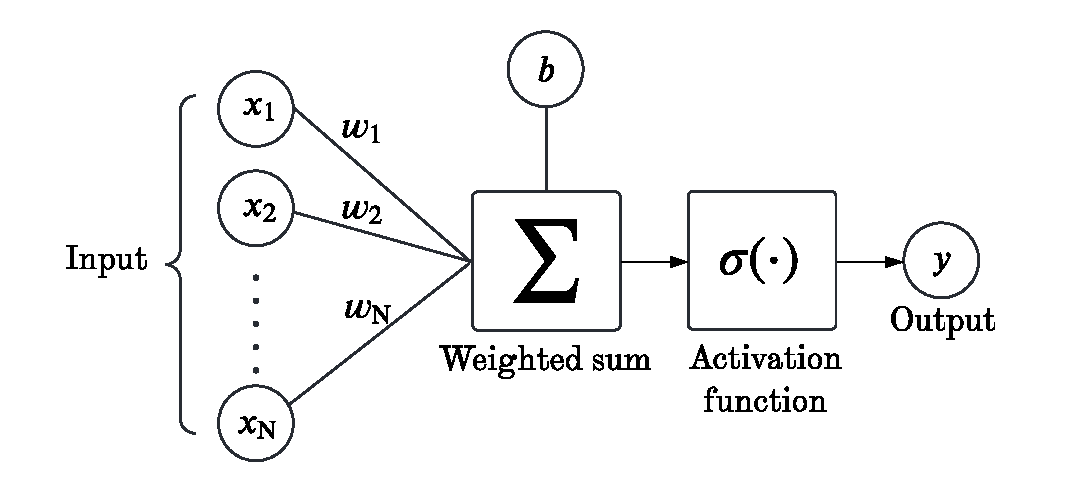
\includegraphics[width=0.57\textwidth]{img/theoretical_background/nn_unit.pdf}
    \caption{The output of a node is computed by applying a non-linear
    activation function $\sigma$ to the weighted sum of its inputs $\bm{x}$ plus
    a bias term $b$.}
    \label{fig:nn_node}
\end{figure}

\begin{definition}[\emph{Neural network parametrization}]
    Let $\bm{x}_k \in \mathbb{R}^{d_k}$ be the input to the layer $k \leq M$, and 
    let $\bm{W} \in \mathbb{R}^{d_k \times d_{k+1}}$ be the $k$-th weight matrix. 
    The output of the layer can be expressed as
    
    $$
    \bm{x}_{k+1} = \sigma_k(\bm{z}_{k+1}) = \sigma_k(\bm{W}_k^T \bm{x}_k + \bm{b}_k),
    $$
    
    where $\sigma_k$ is the non-linear activation function at layer $k$. We 
    can therefore express the overall transformation of a neural network
    as the composition of its layers:
    
    $$
    f_{\operatorname{NN}}(\bm{x}_0; \gamma) = \bm{x}_{M+1} = \bigcirc_{k=0}^{M} \; \sigma_k(\bm{W}_k^T \bm{x} + \bm{b}_k),
    $$
    
    where $\gamma \in \Gamma \subset \mathbb{R}^{|\Gamma |}$ represents the set of parameters 
    of the network. Therefore, the function class $\mathcal{F}$ can be parametrized as $\mathcal{F}_{\Gamma}$ 
    through neural network arquitectures:

    $$
        \begin{aligned}
            \text{NN}: \Gamma & \subseteq \mathbb{R}^{|\Gamma |} \longmapsto \mathcal{F}_{\Gamma} \\
            \gamma & \longmapsto f_{\text{NN}}(\bm{x}; \gamma),
        \end{aligned}
    $$

    where $\Gamma$ is the parameter space navigated by this particular architecture. The function
    class $\mathcal{F}_{\Gamma}$ consists of all mappings $f(\cdot; \gamma): \mathcal{X} \longmapsto \mathcal{Y}$ that 
    that can be realized by some configuration $\gamma \in \Gamma$.
\end{definition}

In order to solve the learning problem, the optimization algorithm must navigate the non-convex loss
landscape towards the minimum of the empirical risk. This is computationally achieved 
by means of gradient-descent-based optimizers, which efficiently compute the
gradient over the parameters via through backpropagation algorithm 
\cite{rumelhartLearningRepresentationsBackpropagating1986}. In practice, more efficient
variations of gradient descent are used, such as stochastic gradient descent (SGD)
\cite{ruderOverviewGradientDescent2017} 
or Adam 
\cite{kingmaAdamMethodStochastic2017}. \\


% \subsection{Backpropagation and gradient descent}

% Let $w_{ji}^{(k)}$ be the weight from node $j$ on layer $k-1$ to node $i$ on layer $k$. Let $a_i^{(k-1)}$ be the output of node $i$ on layer $k-1$ and let $z_j^{(k)} = \sum_{i=0}^{n_k - 1} w_{ji}^{(k)} a_i^{(k-1)} + b_k^{(k)}$ be 
% the linear input of node $j$ on layer $k$, so that $a_j^{(k)} = \sigma_j(z_j^{(k)})$ is the ouput from node $j$. We can compute the gradient of the loss $L$ with respect to the weights by means of the chain rule as follows: 

% $$  
% \frac{\partial L}{\partial w_{ji}^{(k)}} = \frac{\partial L}{\partial a_{j}^{(k)}} \frac{\partial a_{j}^{(k)}}{\partial z_{j}^{(k)}} \frac {\partial z_{j}^{(k)}} {\partial w_{ji}^{(k)}} =
% \frac{\partial L}{\partial a_{j}^{(k)}} \frac{\partial \sigma_j^{(k)}}{\partial z_{j}^{(k)}} a_i^{(k-1)}
% $$

% Given that the loss is computed as a function of the output of the network, all the edges from node $i$ of layer $k-1$ influence the loss value at that node:

% $$
% \frac{\partial L}{\partial a_{i}^{(k-1)}} = \sum_{j=0}^{n_{k} - 1} \frac{\partial L}{\partial a_{j}^{(k)}}  \frac{\partial a_{j}^{(k)}}{\partial z_{j}^{(k)}} \frac{\partial z_{j}^{(k)}}{\partial a_{i}^{(k-1)}} =
% \sum_{j=0}^{n_{k} - 1} \frac{\partial L}{\partial a_{j}^{(k)}} \frac{\partial \sigma_j^{(k)}}{\partial z_{j}^{(k)}} w_{ji}^{(k)}
% $$

% All in all, we see that the same terms are required in different nodes to compute the gradient, making backpropagation algorithm very efficient. Equivalently, for the bias term:

% $$
% \frac{\partial L}{\partial b_{j}^{(k)}} = \frac{\partial L}{\partial a_{j}^{(k)}} \frac{\partial a_{j}^{(k)}}{\partial z_{j}^{(k)}} \frac {\partial z_{j}^{(k)}} {\partial b_{j}^{(k)}} = \frac{\partial L}{\partial a_{j}^{(k)}} \frac{\partial \sigma_j^{(k)}}{\partial z_{j}^{(k)}}
% $$

% These derivatives are the components of the gradient vector that will be used to update the weights and biases of the network.

% $$
% w_{ji}^{(k)} = w_{ji}^{(k)} -\eta \frac{\partial L}{\partial w_{ji}^{(k)}}
% $$

% $$
% b_{j}^{(k)} = b_{j}^{(k)} -\eta \frac{\partial L}{\partial b_{j}^{(k)}}
% $$

% where $\eta$ is the learning rate. More efficient variations of gradient descent such as stochastic gradient descent or Adam are used in practice.


% \subsection{Loss landscape and parameter space}

The universal approximation theorem states that arbitrarily wide architectures
are able to represent virtually any function, but it is an open challenge to theoretically describe which
complexity measure regulates generalization. A possible approach to this problem is to
study the geometry of the loss landscape, especially in the vicinity of local minima. For instance, 
connected flat minima are often associated to better generalization capabilities, as they
intuitively represent a robust region in the parametrization space and should be 
preferred over sharp minima
\cite{jimenezInductiveBiasDeep}. \\

In this work we will explore a different approach to the generalization problem, rooted on
a measure of generalization error that accounts for the implicit randomness of the data
generation process.

\section{Posterior agreement}

As mentioned at the start of the chapter, the input of learning algorithms are
datasets containing observations of a random variable $X$ with support $\mathcal{X}$. The implicit randomness embedded 
in the sampling process extends to the learning outcome of algorithms,
even when performing a deterministic set of operations. 
An alternative intuition of generalization arises from this perspective, in the sense 
that a good algorithm should be expected to learn the same function when trained on 
different realizations of the same experiment (e.g. $\bm{x^\prime}, \bm{x^{\prime\prime}} \sim \bm{X}$). Each
resulting dataset is drawn from the same probability distribution over the support, 
but entails a different instantiation of the randomness associated with the 
sampling process \cite{buhmannDataScienceAlgorithms2022}. \\

A regularization principle is derived from this intuition and can be formalized as a
generalization-complexity trade-off by defining generalization as the robustness or stability
of the learned function to sampling randomness. A suitable measure of complexity in this framework
is the informativeness of the function, which represents its ability to learn the patterns in the
data while filtering out the noise. The more expressive (i.e. complex) a function class is,
the higher will be the estimated information content of the data. If the information content is
underestimated, the approximated function will lack the capacity to learn some patterns in
the data, whereas if informativeness is overestimated, it will overfit to the noise and 
thus not generalize to different realizations of the experiment
\cite{chehreghaniInformationTheoreticModel,buhmannInformationTheoreticModel,buhmannInformationTheoreticModel2010}. \\

The robustness-informativeness regularization principle can be enforced from the set 
of outputs of the learned model, when both the distribution of the data over the support 
and the sampling randomness associated to its measurement are accounted for. This section 
will formalize this principle and derive an expression for the minimization of
the generalization error.

\begin{definition}[\emph{Data distribution}]\label{def:data_distribution}
    The (simple) random sample $\bm{X} \overset{\text{iid}}{\sim} X$ entails a measure of probability
    described by the density function $f_{\bm{X}}$:

    $$
     f_{\bm{X}} = \prod_{n=1}^{N} f_{X},
    $$

    where $f_{X}$ is the density function of $X$. We will use $\mathbf{P}_{\bm{x}}$ to refer to the empirical approximation of this distribution; 
    that is, to the distribution of samples $\bm{x} \sim \bm{X}$:

    $$
    \mathbf{P}_{\bm{x}}(x) = \frac{1}{N} \sum_{n=1}^{N} \delta(x - x_n).
    $$

\end{definition}

\begin{definition}[\emph{Sample}]\label{def:sample}
    Let $X$ be a random variable associated with a measure of probability
    in $\mathcal{X}$. Let $\tau \in \mathcal{T}$ be an instantiation of the randomness allowed
    by such measurement. The class of transformations $\mathcal{T}$ is composed
    of the possible experimental conditions for the data sampling 
    process. The dependency of measurement 
    realizations $\bm{x} \sim \bm{X}$ on experimental conditions 
    will be captured by index $\tau$, and we will implicitly consider sample
    
    $$
        \bm{x} := \tau \circ \bm{x}
    $$

    to be a realization of the experiment $\bm{X} \overset{\text{iid}}{\sim} X$ under conditions $\tau$.
\end{definition}

The nature of $\tau$ is subject to different interpretations depending on the experiment
under consideration. In the context of this work, sampling is limited to a finite set of labeled images
that have been pre-selected for the classification task. For instance, the class of possible transformations
$\mathcal{T}$ defining samples in MNIST \cite{lecun1998mnist} should a priori not include 
the full range of variations that each digit can encompass, since the data collection 
experiment has already been performed. Instead, it would contain the set of possible subsets 
of $N$ images that can be drawn from the MNIST repository, as this reflects the 
true randomness to which the model is pushed to be invariant. \\

Nevertheless, the goal of the learning task is not to generalize within MNIST, but rather
to distill those features in the data that allow the model to generalize to other similar digit observations
that could be collected in the future. For that reason, we will interpret $\tau$ as an instance of the
randomness entailed by the data collection process, which is defined over the (infinite) support 
containing all possible images that can be generated under certain experimental conditions. 
Then, the true data distribution encapsulates the sampling probability of all image features 
that can be possibly generated, and as a consequence the information content of these features for
the task at hand. \\

A dataset generated from $\bm{x} \sim \bm{X}$ entails an instantiation $\tau \in \mathcal{T}$ that 
remains unobserved, since the statistical model governing the data generation process is 
inaccessible. This implies that the information content of the features present in the sample
must be approximated. The suitability of this approximation
will ultimately determine the generalization capabilities of the model. \\

\subsection{Posterior distribution}

%The approximating function $f \in \mathcal{F}$ has been defined as a mapping 
%$\mathcal{X} \longmapsto \mathcal{Y}$, in the sense that an observation $x \in \mathcal{X}$ is mapped to
%a prediction $f(x) \in \mathcal{Y}$. A subtle abuse of notation will be made when considering
%5$f$ to be a 

% THIS IS NOT TRUE
% The data informativeness approximation entailed by the model depends fundamentally
% on the nature of the learning problem, since different tasks will demand different levels of
% informativeness. In the supervised learning framework, we can analogously consider a target 
% information content, which refers to the informativeness of the true mapping of the dataset 
% class. The quality of the approximation will be thus given by the alignment of the informativeness
% attributed to the data with the target information content, which .


% Following this intuition, the robustness of a model will be given by 
% its stability under different noise instantiations,  which is maximum when samples containing the same information are mapped to the same 
% output.

\begin{definition}[\emph{Hypothesis class}]\label{def:hypothesis_class}
    Let $\mathcal{D}$ be the class of supervised datasets generated from $\bm{X}$. 
    A data science algorithm learns a function $f$ implementing the following mapping:

    $$
    \begin{aligned}
        f: \mathcal{D} & \longmapsto \Theta \\
        \bm{x}  & \longmapsto (f(x_1), \dots, f(x_N)) = \theta.
    \end{aligned}
    $$

    The hypothesis class $\Theta$ is the output space of hypothesis representing all 
    possible outcomes of a function $f$ learned on a dataset sampled from $\bm{X}$
    \cite{buhmannDataScienceAlgorithms2022}.

\end{definition}

Intuitively, this framework interprets complexity from the perspective of the set of possible
outcomes of the function, rather than the function class itself. It can be argued
that both perspectives are equivalent, in the sense that any function class can be 
ultimately mapped to a specific hypothesis space $\Theta$. Nevertheless, the underlying transformation is not
homeomorphic in general, and more suitable generalization regularization
constraints can be defined in $\Theta$, especially when dealing with intractable
function classes $\mathcal{F}_{\Gamma}$ represented by deep neural networks. \\

For instance, complexity in the hypothesis class can be associated to the nature of the
randomness displayed by $X$. Ideally, too restrictive hypothesis classes that lack desirable
hypothesis for some realization $\bm{x} \sim \bm{X}$ should be avoided, and also those hypothesis
classes containing unrealizable elements (i.e. hypothesis that are not outcome of
any possible realization of the experiment). A richness condition for the construction of $\Theta$ 
can thus be postulated following this intuition. \\

\begin{proposition}[\emph{Richness condition}]
    $\Theta$ should stem from a
    sufficiently rich set of experimental conditions $\mathcal{T}$ such that every hypothesis $\theta \in \Theta$
    is the outcome of some realization $\bm{x} \sim \bm{X}$.

    $$
    \forall \theta, \exists \tau \in \mathcal{T} \text{ such that } f(\bm{x}) = \theta
    $$
\end{proposition}

Definition \ref{def:sample} states that each datasets entails an instantiation of the sampling 
experiment, which can be formalized as an implicit index $\tau \in \mathcal{T}$ associated with a 
specific realization of the data generation process. The cardinality of $\mathcal{T}$ 
defines an upper bound on the resolution of the hypothesis class, in the sense that no more 
than $|\mathcal{T}|$ different hypothesis will be navigated by a learner, regardless of the task at hand. \\


The richness condition formalizes this intuition by constructing $\Theta$ as a surjective transformation 
of $\mathcal{T}$. As a consequence, the output of the model can be effectively interpreted as a random
variable $\theta$ associated with a measure of probability $\mathbf{P}^f$ over $\Theta$. \\

\begin{definition}[\emph{Posterior}]\label{def:posterior}
    Let $\mathfrak{P}^f$ be a family of distributions under consideration.
    A probability distribution over the hypothesis class can be defined as a 
    conditional distribution given an realization $\bm{x} \sim \bm{X}$. 
    We will refer to this distribution as the posterior over $\Theta$ under $f$:

    $$
        \begin{aligned}
            \mathbf{P}^f: \mathcal{D} \times \Theta & \longmapsto \mathbb{R} \\
            (\bm{x}, \theta) & \longmapsto \mathbf{P}^f (\theta \mid \bm{x}).
        \end{aligned}
    $$

    The posterior $\mathbf{P}^f \in \mathfrak{P}^f$ establishes the stochastic relation between data realizations and hypotheses.
    
\end{definition}

Using these definitions we can operate over $\Theta$ within the framework of probability 
theory. For instance, we can obtain the (prior) probability of a hypothesis to be
selected by $f$ as

$$
 \Pi^f (\theta) = \mathbb{E}_{\mathcal{T}} \; \mathbf{P}^f (\theta \mid \tau) = \mathbb{E}_{\bm{X}} \; \mathbf{P}^f (\theta \mid \bm{x}),
$$

from which we can derive a probabilistic version of the richness condition, where a limit
case can be imposed with exactly one experiment per hypothesis, leading to a uniform prior

$$
\Pi^f (\theta) = |\Theta|^{-1}
$$

when the hypothesis class is finite. Within this framework, selecting suitable hypothesis classes amounts to selecting
posterior distributions that yield a higher probability to the desired subset of hypothesis. This
is the leading principle that will guide the derivations that follow.

\subsection{Generalization error}

In order to postulate an informativeness-based definition of generalization error, we will consider
two samples $\bm{x}', \bm{x}'' \sim \bm{X}$ generated from the same experiment. Samples are independent in
general and they only differ in the implicit randomness entailed by the sampling experiment:

$$
    \mathbf{P}_{\bm{x}', \bm{x}''} = \mathbf{P}_{\bm{x}'} \mathbf{P}_{\bm{x}''}.
$$

\begin{proposition}[\emph{Posterior selection principles}]
    Let $\mathcal{T}_{\bm{X}} \subseteq \mathcal{T}$ be the subset of sampling realizations 
    that is effectively navigated by $\bm{X}$, in the sense that it encompasses only those instantiations
    that can be sampled from $\bm{X}$. Let $\Theta_{\bm{X}} \subseteq \Theta$ be the realizable 
    subset\footnote{
        \flushbottom In the context of supervised classification tasks, $\mathcal{T}_{\bm{X}} \subseteq \mathcal{T}$ and 
        therefore $\Theta = \Theta_{\bm{X}}$, since the number of classes
        is fixed beforehand and all possible combinations of labels are realizable a priori.
    } 
    of hypotheses, generated as a surjective transformation of $\mathcal{T}_{\bm{X}}$. Following
    the intuition introduced at the beginning of the chapter, two posterior selection principles are 
    derived from the robustness-informativeness trade-off:
    % \vspace{-1.5mm}
    \begin{itemize}
        \item Posteriors $\mathbf{P}^f$ should be expressive enough to cover the realizable subset $\Theta_{\bm{X}}$.
        \vspace{-2.5mm}
        \item Equally likely inputs drawn from the same experiment should yield similar sets of hypothesis.
    \end{itemize}
\end{proposition}


% Two posterior selection principles are derived from the robustness-informativeness trade-off:
% \vspace{-1.5mm}
% \begin{description}
%     \item[P1] Posteriors $\mathbf{P}^f$ should be expressive enough to cover the realizable subset of $\Theta$.
%     \vspace{-2.5mm}
%     \item[P2] Equally likely inputs drawn from the same experiment should yield similar sets of hypothesis.
% \end{description}

% Two posterior selection principles are derived from the robustness-informativeness trade-off:
% \vspace{-2mm}
% \begin{itemize}
%     \item Posteriors should be expressive enough to cover the realizable subset of the hypothesis space.
%     \vspace{-3mm}
%     \item Equally likely inputs drawn from the same experiment should yield similar sets of hypothesis.
% \end{itemize}

\begin{definition}[\emph{Description length}]
    Let $\mathcal{F}_{\Gamma}(\cdot)$ be the function class encompassing all functions 
    represented by a parametrization $\Gamma$. Let $\mathbf{P}_{\Gamma}$ be the
    universal distribution relative to $\mathcal{F}_{\Gamma}$ fulfilling the minimum
    description length principle. The description length of a function $f_\gamma \in \mathcal{F}_{\Gamma}$ 
    is defined as the number of bits required to encode its parameters
    \cite{grunwaldMinimumDescriptionLength2019}.
    The code length of the argument of such distribution is

    $$
    \text{DL}_{f_{\gamma}}(\cdot) = -\log f_{\gamma}(\cdot).
    $$
\end{definition}

The quality of the represented function $f$ will be measured by the description
length of its posterior \cite{buhmannDataScienceAlgorithms2022}, and 
thus a loss function can be defined as follows:

$$
    \ell (\theta, \bm{x}) = - \log \mathbf{P}^f (\theta \mid \bm {x}).
$$

Given that description length also accounts for the complexity of the hypothesis
class and not only its generalization capabilities, loss values are normalized by
dividing by the description length of the prior:

$$
    - \log \Pi^f (\theta) = - \log \mathbb{E}_{\bm{X}} \mathbf{P}^f (\theta \mid \bm{x}).
$$

\begin{definition}[\emph{Generalization error}]
    Let $\bm{x'}$ and $\bm{x''}$ be realizations of $\bm{X}$.
    Let $\Theta$ be the (realizable) hypothesis class represented by $f$ given $\bm{X}$. 
    The generalization error is defined as the out-of-sample description length:

    $$
        \mathcal{G}_{\mathcal{X}} = \mathbb{E}_{\bm{x}', \bm{x}''} \mathbb{E}_{\mathbf{P}^f( \theta \mid \bm{x}')} \left[ - \log \frac{\mathbf{P}^f(\theta | \bm{x}'')}{\Pi^f (\theta)} \right].
    $$
    
\end{definition}

It amounts to the expected loss over the normalized posteriors on (validation) sample
$\bm{x}''$ weighted over the posterior distribution on (training) sample $\bm{x}'$.
Intuitively, a lower generalization error is achieved when good quality hypothesis
on $\bm{x}''$ are likely to be drawn from $\bm{x}'$. 


\begin{lemma}[\emph{Posterior agreement}]\label{lemma:pa}
    The generalization error $\mathcal{G}_{\mathcal{X}}$ is non-negative and has a lower bound $-\mathcal{J}$. 
    \textcolor{blue}{We define $\mathcal{J}$ as the posterior agreement.}
\end{lemma}
\begin{proof}
    $$
    \begin{aligned}
        \mathcal{G}_{\mathcal{X}} & \geq \mathbb{E}_{\bm{x}', \bm{x}''}\left[-\log \left(\mathbb{E}_{\mathbf{P}^f( \theta \mid \bm{x}')} \frac{\mathbf{P}^{f}\left(\theta \mid \bm{x}''\right)}{\Pi^{f}(\theta)}\right)\right] \\
        & = \textcolor{blue}{\boxed{\mathbb{E}_{\bm{x}', \bm{x}''} \left[-\log \left(\sum_{\theta \in \Theta} \frac{\mathbf{P}^{f}\left(\theta \mid \bm{x}'\right) \mathbf{P}^{f}\left(\theta \mid \bm{x}'' \right)}{\Pi^{f}(\theta)}\right)\right] = -\mathcal{J}}} \\
        & \geq-\log \left(\mathbb{E}_{\bm{x}', \bm{x}''} \mathbb{E}_{\mathbf{P}^f( \theta \mid \bm{x}')} \mathbb{E}_{\mathbf{P}^f(\theta \mid \bm{x}'')} \frac{\mathbf{P}^{f}\left(\theta \mid \bm{x}''\right)}{\Pi^{f}(\theta)}\right)=0,
    \end{aligned}
    $$

where Jensen's inequality has been applied twice to the convex function $-\log$. \\

\end{proof}

\subsection{Maximum posterior agreement}

The maximum posterior agreement criterion, which follows 
from Lemma \ref{lemma:pa}, can be formalized as an optimization problem over the 
function class. See illustration in Figure \ref{fig:illustrate_beta}.

\begin{definition}[\emph{Kullback-Leibler divergence}]
    Let $\mathbf{P}$ and $\mathbf{Q}$ be two probability distributions over the same support $\Theta$. 
    The Kullback-Leibler divergence of $Q(\theta)$ relative to $P(\theta)$ is defined as

    $$
    \text{KL}(\mathbf{P}(\theta) \parallel \mathbf{Q}(\theta)) = \mathbb{E}_{\mathbf{P}(\theta)} \left[ \log \frac{\mathbf{P}(\theta)}{\mathbf{Q}(\theta)} \right].
    $$

\end{definition} 

\begin{definition}[\emph{Cross-entropy}]
    Let $\mathbf{P}$ and $\mathbf{Q}$ be two probability distributions over the same support $\Theta$. 
    The cross-entropy of $\mathbf{Q}(\theta)$ relative to $\mathbf{P}(\theta)$ is defined as

    $$
    H_{\mathbf{P}, \mathbf{Q}} = - \mathbb{E}_{\mathbf{P}(\theta)} \log \mathbf{Q}(\theta)
    $$

\end{definition}

\begin{proposition}[\emph{Posterior agreement criterion}]\label{def:pa}
    The posterior agreement model-selection criterion is defined as follows.

    $$
    \begin{aligned}
        \sup_{\mathcal{F}} & \; \mathcal{J} \\
        \text{s.t.} & \; \text{KL}(\mathbf{\Pi}^f(\theta) \parallel |\Theta|^{-1}) \leq \xi,
    \end{aligned}
    $$
    
    where $\xi \in \mathbb{R}$ represents a small allowed deviation from uniformity in the prior.
\end{proposition}

\begin{theorem}[\emph{Maximum posterior agreement}]
The optimal $\mathbf{P}_{*}^f$ maximizing the posterior agreement criterion defines a lower bound
in the generalization error $\mathcal{G}_{\mathcal{X}}$ under the richness condition:

$$
    \inf_{\mathcal{F}} \mathcal{G}_{\mathcal{X}} \geq -\sup_{\mathcal{F}} \mathcal{J}.
$$
\end{theorem}

\begin{proof}
    We consider the lagrangian formulation of the generalization error minimization problem 
    and apply Lemma \ref{lemma:pa}.

    $$
    \begin{aligned}
        & \inf_{\mathcal{F}} \left \{ \mathcal{G}_{\mathcal{X}} + \alpha \text{KL} (\mathbf{\Pi}^f(\theta)) \parallel |\Theta|^{-1} \right \} \\
        = & \; \inf_{\mathcal{F}} \left \{ \mathcal{G}_{\mathcal{X}} + \alpha \mathbb{E}_{\mathbf{\Pi}^f(\theta)} \log \mathbf{\Pi}^f(\theta) + \alpha \mathbb{E}_{\mathbf{\Pi}^f(\theta)} \log |\Theta| \right \} \\
        \geq & \; \alpha \log |\Theta| + \inf_{\mathcal{F}} \left \{ \alpha H_{\mathbf{\Pi}^f} \right \} - \sup_{\mathcal{F}} \left \{ \mathcal{J} \right \} \\
        \geq & \; - \sup_{\mathcal{F}} \mathcal{J}
    \end{aligned}
    $$

    % The last inequality follows from the fact that the entropy does not exceed the log-cardinality
    % of the hypothesis class:

    % $$
    % H_{\mathbf{\Pi}^f}(\theta) \leq \log |\Theta|, \;\; \forall \mathbf{\Pi}^f.
    % $$

    The last inequality follows from the fact that the entropy does not exceed the log-cardinality
    of the hypothesis class, $H_{\mathbf{\Pi}^f}(\theta) \leq \log |\Theta|, \;\; \forall \mathbf{\Pi}^f$.
\end{proof}

\begin{figure}[H]
    \centering
    \begin{subfigure}[b]{0.3\textwidth}
        \centering
        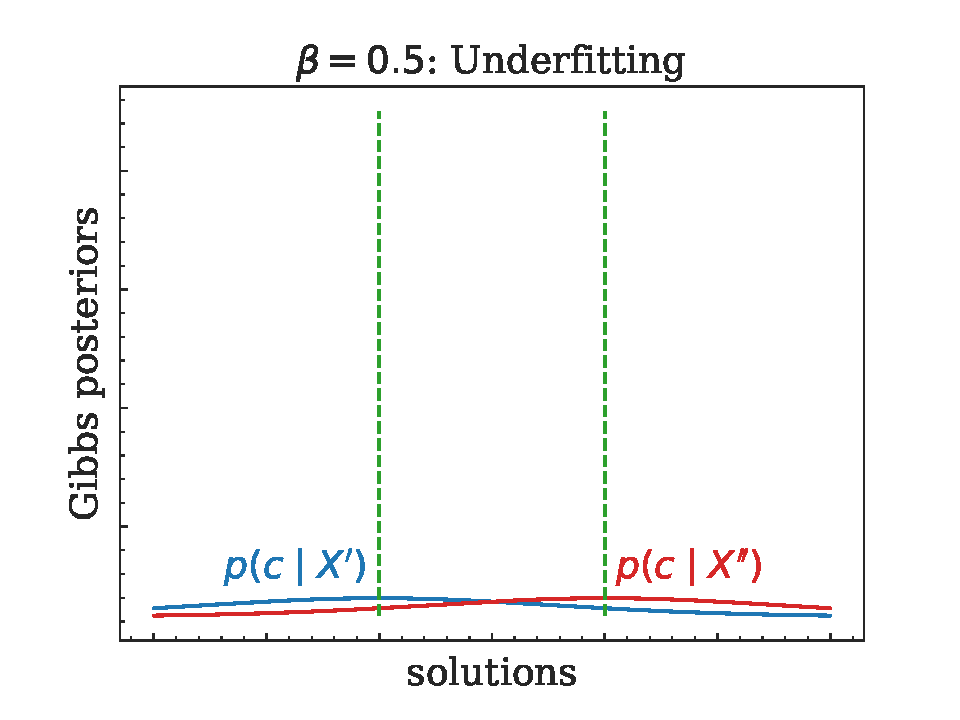
\includegraphics[width=\textwidth]{img/theoretical_background/method_beta=0.5.pdf}
    \end{subfigure}
    \hfill
    \begin{subfigure}[b]{0.3\textwidth}
        \centering
        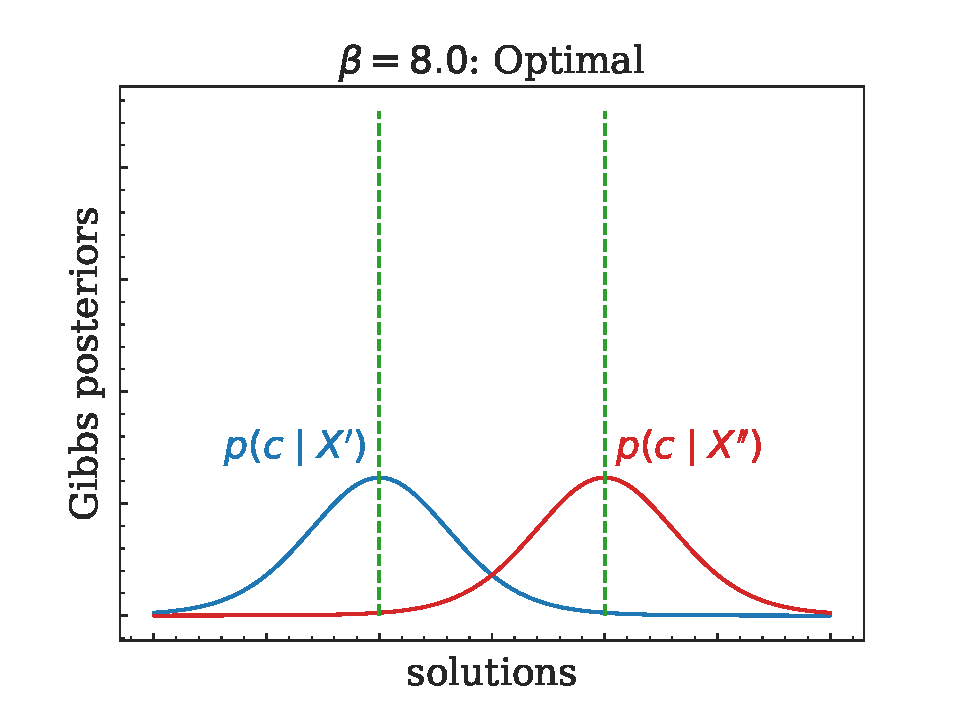
\includegraphics[width=\textwidth]{img/theoretical_background/method_beta=8.0.pdf}
    \end{subfigure}
    \hfill
    \begin{subfigure}[b]{0.3\textwidth}
        \centering
        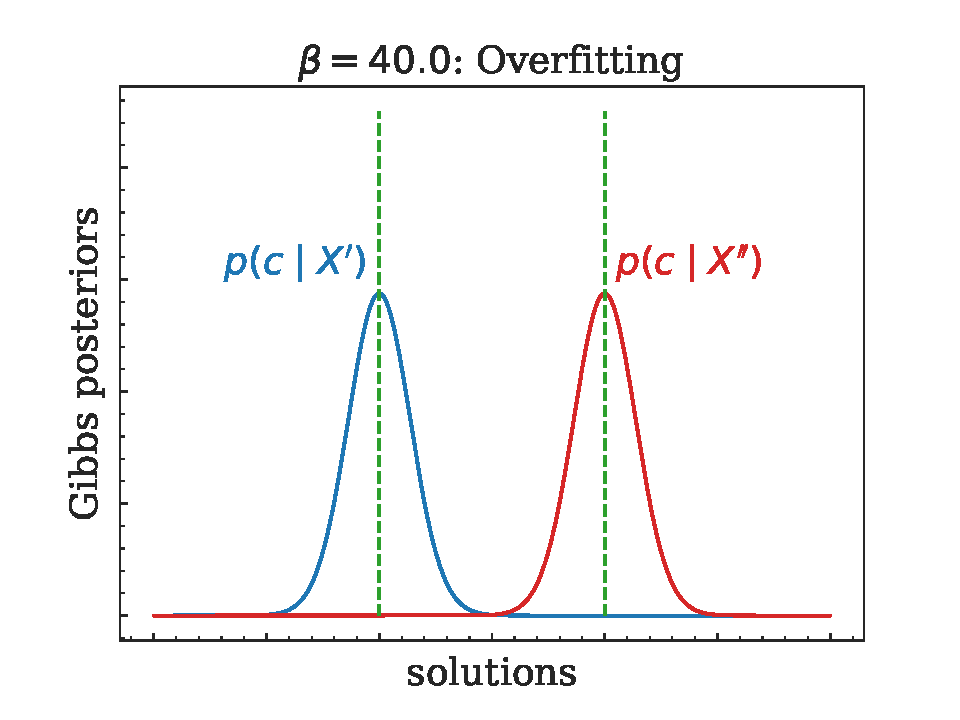
\includegraphics[width=\textwidth]{img/theoretical_background/method_beta=40.0.pdf}
    \end{subfigure}

    \vspace{1em}

    \begin{subfigure}[b]{0.97\textwidth}
        \centering
        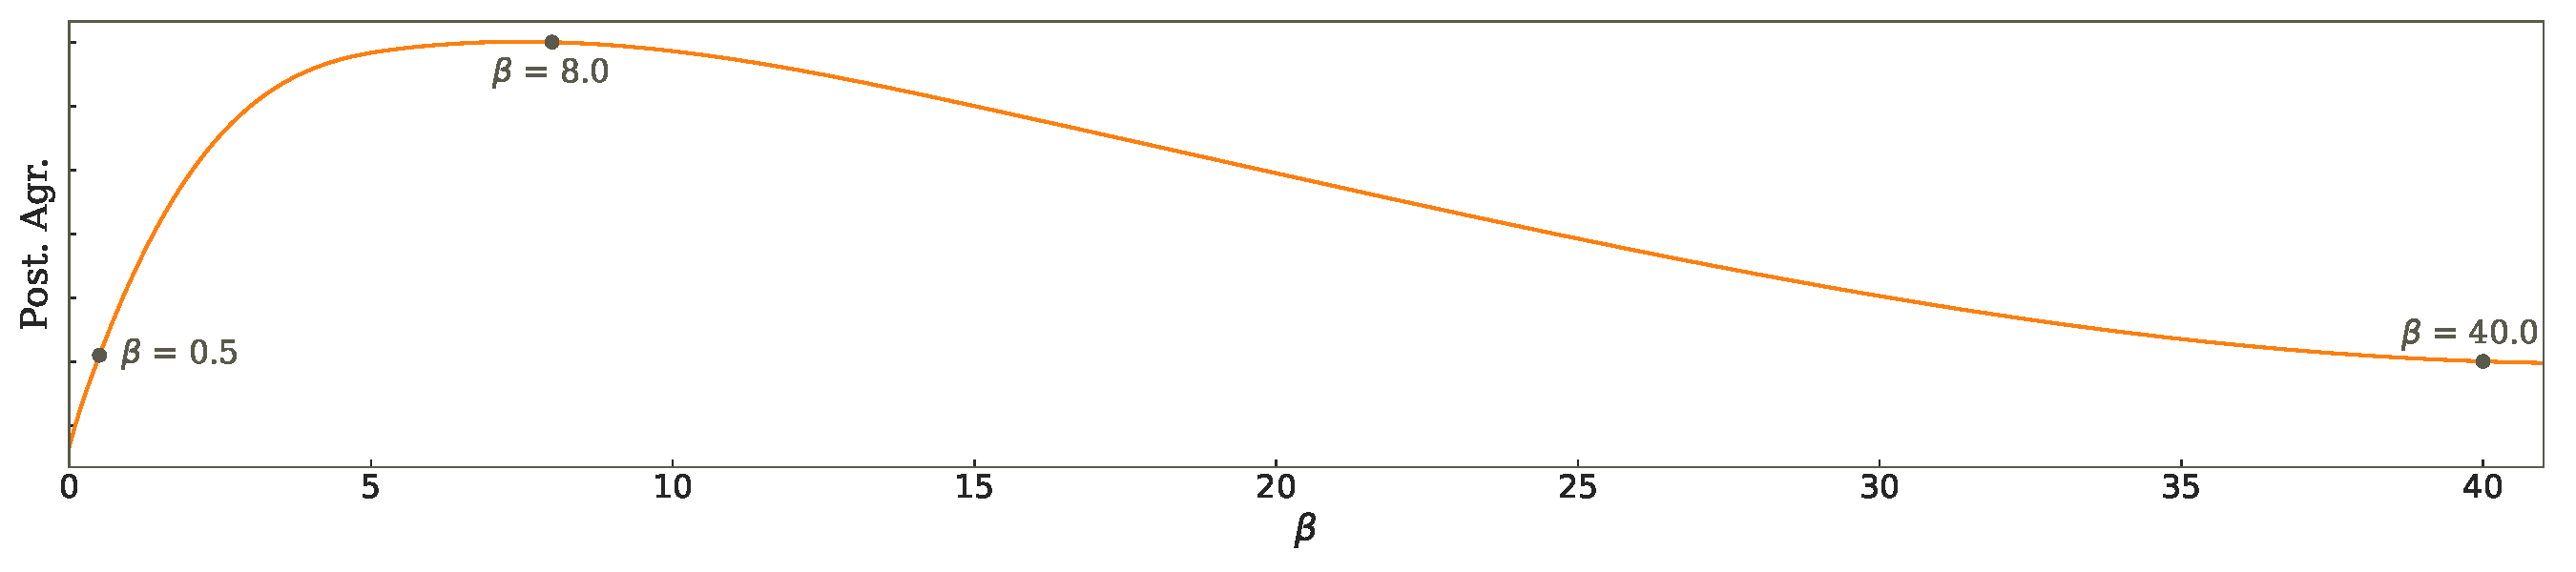
\includegraphics[width=\textwidth]{img/theoretical_background/gibbs_betas.pdf}
    \end{subfigure}

    
    \caption{
        Qualitative illustration of the optimization over the inverse temperature parameter $\beta$. 
        When $\beta \longrightarrow 0$, the informativeness of 
        the posterior is reduced, eventually converging to a uniform distribution. When
        $\beta \longrightarrow \infty$, the informativeness of the posterior grows, leading
        to an increasingly peaked distribution. Posterior Agreement is maximum at a value $\beta^{*}$ 
        in which hypothesis selected from the posterior over $\theta \mid \bm{x^\prime}$ are assigned
        a high probability by the posterior over $\theta \mid \bm{x^{\prime\prime}}$, which in this case
        aligns with the maximum posterior overlap.
        \cite{buhmannDataScienceAlgorithms2022}
    }
    \label{fig:illustrate_beta}
\end{figure}

